\chapter{Fundamentação Teórica}\label{cap:fundamentacao}

Neste capítulo são discutidos os conceitos básicos ao entendimento deste trabalho, abrangendo processamento digital de imagens, segmentação de imagens, aprendizagem de máquina, extração de características e avaliação de desempenho dos métodos utilizados.

\section{Processamento Digital de Imagens}

Uma imagem pode ser definida por uma função bidimensional, $f(x,y)$, onde $x$ e $y$ são coordenadas espaciais de um plano, e a amplitude de $f$ para um par de coordenadas $(x,y)$ é chamada de intensidade da imagem naquele ponto. Quando $x$, $y$ e a amplitude de valores de $f$ representam quantidades finitas e discretas, podemos chamar a imagem de imagem  digital. A linha de pesquisa de processamento digital de imagens se refere ao processamento digital dessas imagens através de um computador digital \cite{gonzalez:2002}.

Uma imagem digital é composta por um número finito de elementos, cada um com um valor ($f$) e localização ($x$ e $y$) particulares. Estes elementos são chamados de elementos da imagem ou \textit{pixels}, do inglês \textit{picture elements}.

Ainda de acordo com \citeonline{gonzalez:2002}, o interesse em processamento digital de imagens advém de duas principais áreas de aplicação: melhoramento de informações pictóricas para interpretação humana; e processamento de imagens para armazenamento e transmissão de dados, e representação para percepção de máquinas autônomas.

Para praticamente qualquer aplicação de processamento de imagens, características destas mesmas imagens precisam ser extraídas. Segundo \citeonline{yadav:2009}, as características de imagens digitais podem ser classificadas em baixo e alto nível. As características de baixo nível são extraídas diretamente das imagens, geralmente descrevendo atributos locais ou de pequenos agrupamentos de pixels. As características de alto nível são extraídas a partir de características de baixo nível, e compreendem informações sobre regiões maiores da imagem, ou mesmo da imagem completa. Na próxima seção, são descritas as características utilizadas neste trabalho.

\subsection{Características de baixo nível}

As características de baixo nível de uma imagem compreendem aspectos técnicos da composição desta imagem. Informações sobre cores, intensidade e bordas de uma imagem são fundamentais para a extração de características de alto nível, mas também são úteis diretamente em diversas tarefas de processamento digital de imagens, tais como segmentação e filtragem.

\subsubsection*{Espaços de cores}

O uso de cores em processamento de imagem é motivado por dois principais fatores. Primeiramente, cor é um poderoso descritor que frequentemente simplifica a identificação e extração de objetos de uma cena. Em segundo lugar, humanos podem discernir milhares de tons e intensidades de cores, comparado com apenas duas dúzias de tons de cinza \cite{gonzalez:2002}.

Os espaços de cores, também conhecidos como modelos de cores ou sistemas de cores, são maneiras padronizadas de representar a cor de pixels em uma imagem digital. A definição do modelo de cores persegue, geralmente, dois propósitos: o hardware ou meio pelo qual a cor será reproduzida (RGB para representação em telas, CMYK para impressão, por exemplo), ou a manipulação de certos elementos da cor, como tom, saturação, etc.

O espaço de cores RGB (\textit{Red, Green, Blue}) é baseado numa representação de coordenadas cartesianas de três canais de cores: vermelho (R), verde (G) e azul (B). Os 3 canais possuem a mesma amplitude, portanto, em uma imagem RGB de 24 bits, cada canal é representado por 8 bits, que pode ter seu valor de 0 a 255.

%Por conta destas características, o espaço de cores RGB é geralmente representado por um cubo (Figura \ref{fig:rgb_cubo}), onde as arestas alinhadas aos eixos X, Y e Z são respectivamente os valores primários de vermelho $(255,0,0)$, verde $(0,255,0)$ e azul $(0,0,255)$. Neste espaço de cores, os tons de cinza partem do ponto preto $(0,0,0)$ e acompanham a diagonal do cubo até o ponto branco (255,255,255).
%
%\begin{figure}[h]
%  \centering
%  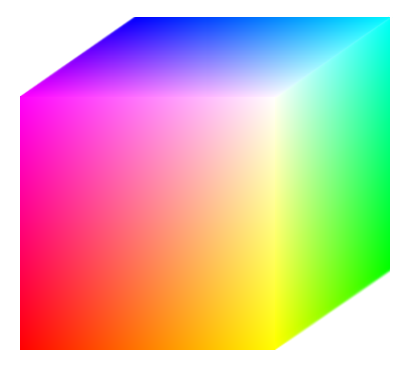
\includegraphics[width=0.4\textwidth]{imgs/rgb_cubo}
%  \caption[Cubo do espaço de cores RGB]{Cubo representando o espaço de cores RGB. Em uma imagem RGB de 24 bits, o cubo possui 16.777.216 cores, $(2^8)^3$. Fonte: \cite{gonzalez:2002}}
%  \label{fig:rgb_cubo}
%\end{figure}

O espaço de cores RGB é ideal para a representação de hardware que combine cores através da mistura de luzes, tais como monitores e projetores. Seus canais são cores, e a combinação deles é intuitiva à composição ou geração de cores, mas é muito pouco intuitiva para seres humanos.

Com esta finalidade, outros espaços de cores podem ser menos intuitivos a seres humanos, mas são definidos de forma que outras características das cores sejam facilmente extraídas. O HSI (\textit{Hue, Saturation, Intensity}), também conhecido como HSV (\textit{Hue, Saturation, Value}) representa uma cor através de seu tom, saturação e intensidade. Este espaço de cores facilita a extração de algumas características como saturação ou intensidade. Seus canais também se parecem mais com a forma como seres humanos descrevem cores, já que um dos canais representa a informação de cor pura, enquanto os outros canais tratam da saturação (força) e itensidade (brilho) da cor. Todos os canais têm seus valores representados por percentuais, com valores decimais de $0$ a $1$.

%O espaço de cores HSI pode ser representado por um cone, onde a altura é definida pela intensidade, o raio é definido pela saturação e a posição na circunferência é definida pelo tom da cor (Figura \ref{fig:hsi_cone}).
%
%\begin{figure}[h]
%  \centering
%  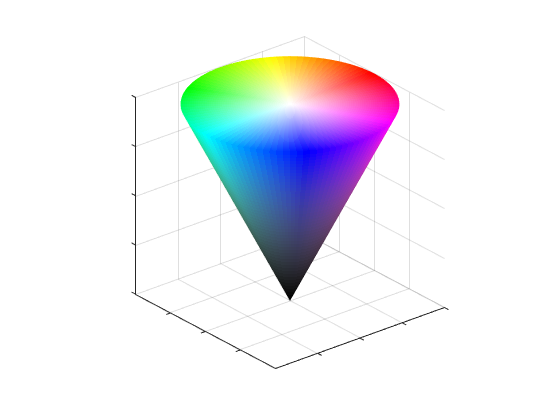
\includegraphics[width=0.8\textwidth]{imgs/hsi_cone}
%  \caption[Cone do espaço de cores HSI]{Cone representando o espaço de cores HSI.}
%  \label{fig:hsi_cone}
%\end{figure}

\subsubsection*{Intensidade}

É comum que se precise extrair a intensidade dos pixels de uma imagem, seja para análise de textura, para composição de histograma ou qualquer outro propósito. Quando a imagem está no espaço de cores HSI, basta que o canal de intensidade (I) seja coletado. Quando se está trabalhando no espaço de cores RGB, uma conversão precisa ser feita:

\begin{equation}
	\displaystyle I = \frac{R + G + B}{3}
	\label{eq:rgb_intensidade}
\end{equation}

onde I é a intensidade do pixel e R, G e B são, respectivamente, os canais vermelho, verde e azul do pixel. Esta fórmula também pode ser utilizada para converter imagens coloridas RGB em imagens em tons de cinza, embora, por características intrínsecas ao sistema de visão humano, normalmente alguns pesos diferentes são atribuídos ao canais quando o objetivo é a visualização humana da imagem, ao invés da média aritmética simples da equação \ref{eq:rgb_intensidade}, que é considerada pela literatura uma aproximação suficientemente adequada para sistemas de visão computacional.

\subsection{Características de alto nível}

Muitas vezes, características de baixo nível não são suficientes para descrever aspectos da imagem a ser processada. Especialmente em tarefas de visão computacional, é muito comum que seja necessário extrair características ou conceitos a partir de características de baixo nível. Informações de textura, morfologia e pontos de interesse são algumas destas características.

\subsubsection*{Textura}

De acordo com \citeonline{nixon:2008}, não há uma definição formal de textura. \citeonline{gonzalez:2002}, por sua vez, definem textura como uma medida de propriedades sensoriais como maciez, coesão e regularidade. Um campo de pesquisa que constantemente apresenta novidades substanciais, as soluções para descrição e extração de texturas em imagens digitais partem de duas principais abordagens: estatística e  espectral.

A abordagem estatística consiste no uso de modelos estatísticos do histograma de intensidade de uma imagem ou de uma porção dela. Seja $z$ uma variável que representa uma intensidade e $p(z_i), i = 0, 1, 2,..., L$, onde $L$ é o número de intensidades distintas na região investigada, o n-ésimo momento de $z$ pode ser definido por:

\begin{equation}
	\displaystyle \mu_n(z) = \sum_{i=0}^{L-1} (z_i - m)^n p(z_i)
\end{equation}

onde $m$ é o valor médio de $z$:

\begin{equation}
	\displaystyle m = \sum_{i=0}^{L-1} z_i p(z_i)
\end{equation}

A partir disto, medidas de maciez relativa podem ser extraídas, medindo a variância entre diferentes momentos estatísticos do histograma ($z, z+1, z+2...$). A literatura está repleta de exemplos desta abordagem, se utilizando de atributos como a entropia média (equação \ref{eq:textura_entropia}) ou uniformidade (equação \ref{eq:textura_uniformidade}).

\begin{equation}
	\displaystyle e(z) = - \sum_{i=0}^{L-1} p(z_i) \log_2 p(z_i)
	\label{eq:textura_entropia}
\end{equation}

\begin{equation}
	\displaystyle U(z) = \sum_{i=0}^{L-1} p^2(z_i)
	\label{eq:textura_uniformidade}
\end{equation}

A descrição e extração de texturas seguindo uma abordagem espectral consiste na transformação da imagem para o domínio de frequência, através da transformada de Fourier, e o posterior agrupamento das informações de frequência a fim de obter algumas métricas ou descritores das texturas. A principal desta abordagem é sua invariância à aspectos espaciais. Desta forma, padrões de variação de intensidade nas imagens podem ser visualizados e extraídos (figura \ref{fig:textura_fourier}).

\begin{figure}[h]
  \centering
  \begin{subfigure}[b]{0.45\textwidth}
    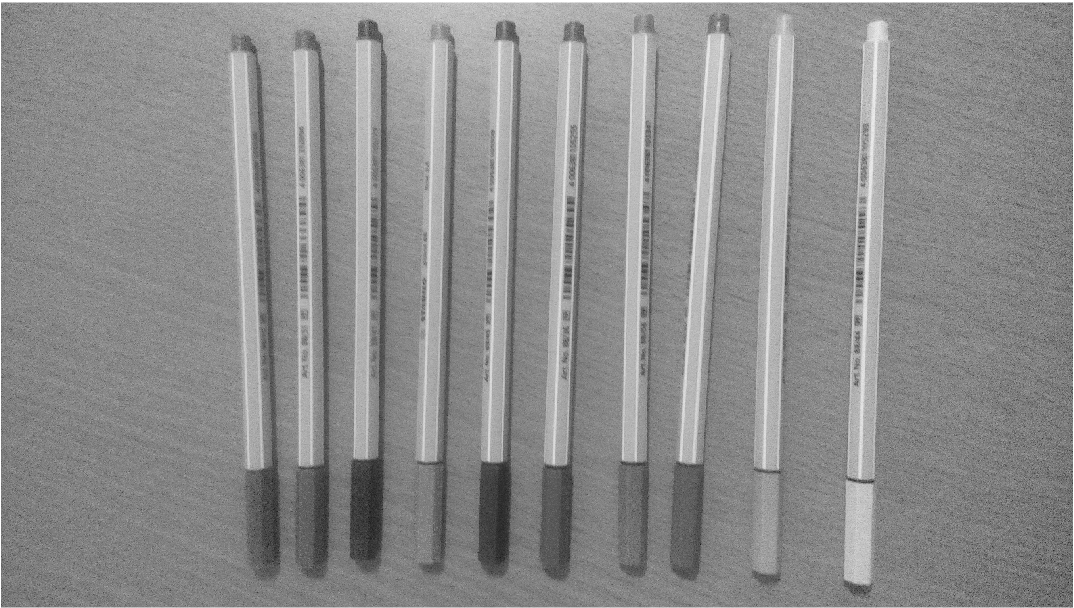
\includegraphics[width=\textwidth]{imgs/stab_1}
  \end{subfigure}%
  ~
  \begin{subfigure}[b]{0.45\textwidth}
    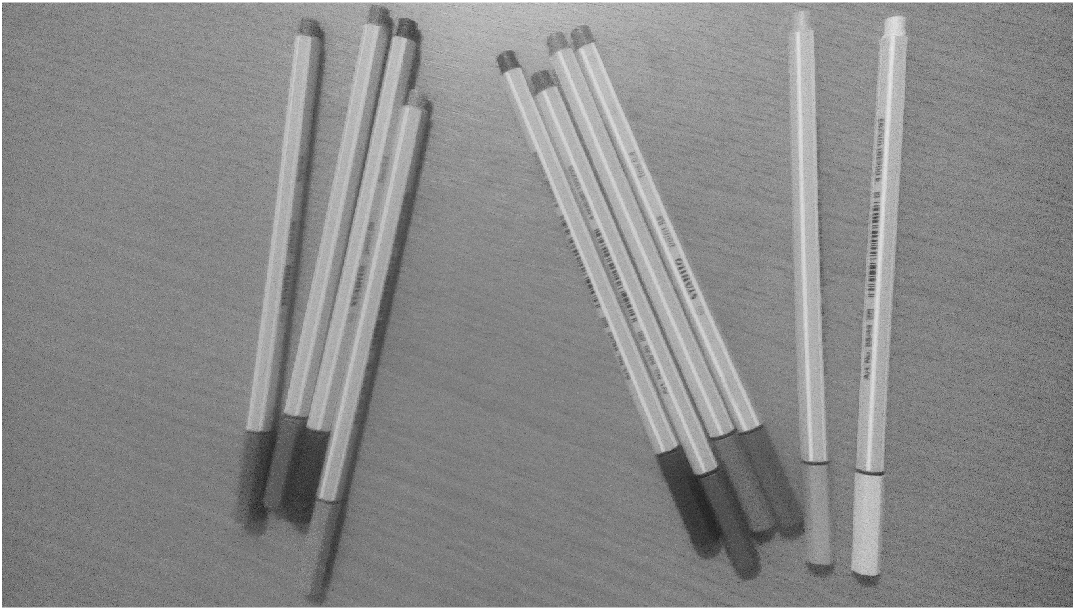
\includegraphics[width=\textwidth]{imgs/stab_2}
  \end{subfigure}%
  \\
  \begin{subfigure}[b]{0.45\textwidth}
    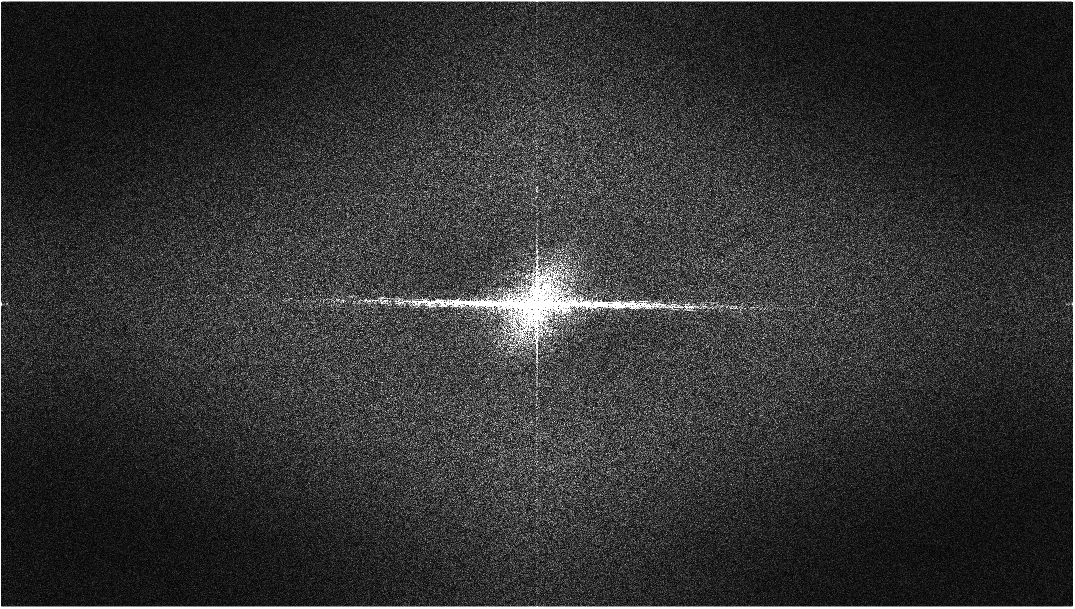
\includegraphics[width=\textwidth]{imgs/stab_1_spectra}
  \end{subfigure}%
  ~
  \begin{subfigure}[b]{0.45\textwidth}
    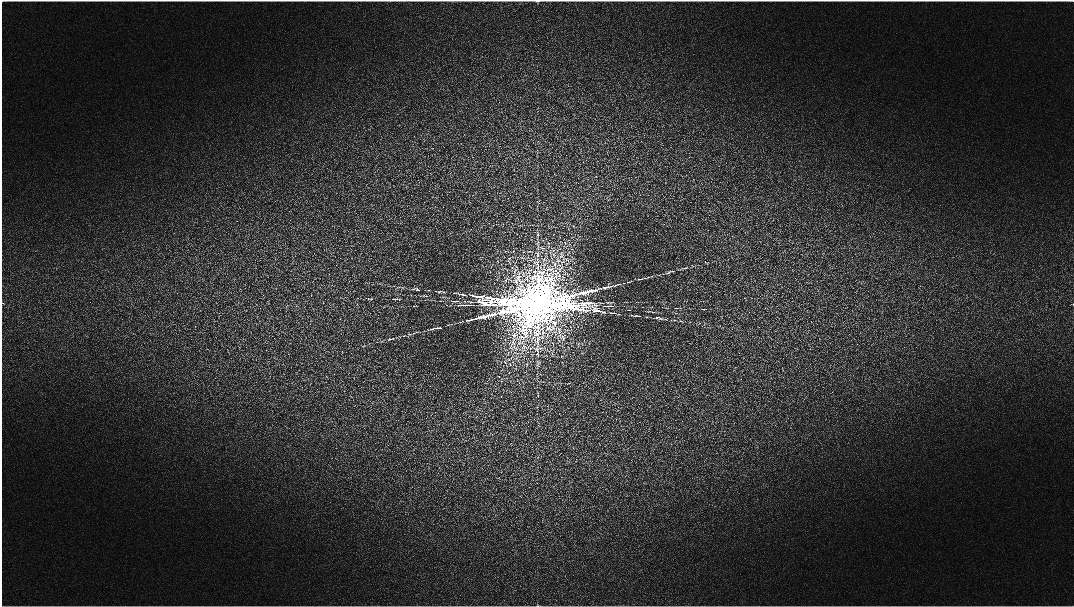
\includegraphics[width=\textwidth]{imgs/stab_2_spectra}
  \end{subfigure}%
  \caption[Exemplo de extração de texturas utilizando transformada de Fourier]{Exemplo de extração de texturas utilizando transformada de Fourier. As imagens inferiores são representações gráficas do espectro de frequência de intensidade das imagens acima}
  \label{fig:textura_fourier}
\end{figure}

Um dos modelos mais populares e descritivos de características de textura com abordagem espectral é o Local Binary Pattern (LBP), introduzido por \citeonline{ojala:1994}. Em primeiro lugar, este modelo divide a região examinada em células, normalmente cada célula corresponde a um pixel. Em seguida, cada célula é comparada com suas oito células vizinhas, e a diferença de intensidade (um valor binário que simboliza "maior" ou "menor") é utilizada para construir uma máscara de 8 bits, que serve como uma espécie de impressão digital daquela célula na região examinada. A junção da máscara de todas as células compõe o que é chamado de Padrão Binário Local (LBP) da região, uma característica de alta dimensionalidade, mas bastante descritiva.

Diversas variações de LBP existem na literatura, algumas visando melhorar a descrição de certos aspectos da imagem, outras almejando a invariância de rotação ou escala da imagem. Como será visto no capítulo \ref{cap:trabalhos}, este tipo de descritor é comumente usado em trabalhos de classificação de imagens.

\subsubsection*{Morfologia}

Segundo \citeonline{nixon:2008}, parte importante da extração de características de alto nível em imagens é a busca por formas e padrões. As abordagens para extrair formas de imagens vão desde as mais simples, como a limiarização, que faz análise pixel a pixel da imagem para tentar separar o componente principal do fundo da imagem (todo o resto que não interessa à análise), passando pelo casamento de padrões, que se utiliza de uma amostra da forma desejada para realizar a busca pelo mesmo padrão na imagem, até poderosos extratores de formas geométricas como a transformada de Hough.

A transformada de Hough, introduzida por \citeonline{hough:1962} é uma técnica criada para extrair formas geométricas de imagens. O objetivo desta técnica está na descrição da imagem ou região através de retas, círculos e elipses presentes na mesma. Inicialmente concebida para detectar apenas linhas em diversos ângulos, atualmente todas as implementações e variações da transformada Hough derivam do trabalho de \citeonline{duda:1972}, responsáveis pela criação da transformada de Hough generalizada, capaz de detectar os demais círculos e elipses. Desde então, diversas melhorias têm sido feitas para acelerar o algoritmo, bem como suportar a detecção de formas geométricas arbitrárias.

Para detectar linhas em imagens utilizando a transformada Hough, é preciso, primeiramente, compreender que em uma abordagem cartesiana, pontos colineares em uma imagem estão relacionados pela inclinação $m$ e um ponto de interceptação $c$, de forma que:

\begin{equation}
	\displaystyle y = mx + c
\end{equation}

ou, reescrevendo a equação de forma linear homogênea:

\begin{equation}
	\displaystyle Ay + Bx + 1 = 0
\end{equation}

onde $A = -1/c$ e $B = m/c$.

Dado que um par de coordenadas $(x,y)$ define uma reta no espaço com parâmetros $(A,B)$, podemos dizer que a equação é simétrica. Se ${(x_i,y_i)}$ é um conjunto de pontos lineares que definem a reta $(A,B)$, temos que:

\begin{equation}
	\displaystyle Ay_i + Bx_i + 1 = 0
\end{equation}

Esta equação pode ser vista como um sistema de equações e pode ser reescrita em termos de parametrização cartesiana:

\begin{equation}
	\displaystyle c = -x_im + y_i
\end{equation}

Com a finalidade de encontrar linhas retas na imagem, a transformada de Hough busca satisfazer as incógnitas desta equação, utilizando também parâmetros externos para determinar tolerância de inclinação e comprimento mínimo das retas.

De forma similar, a transformada de Hough busca por círculos que satisfaçam:

\begin{equation}
	\displaystyle (x-x_0)^2 + (y-y_0)^2 = r^2
\end{equation}

que, convertida para forma paramétrica, temos:


\begin{equation}
	\displaystyle x = x_0 +r \cos(\theta)
\end{equation}

\begin{equation}
	\displaystyle y = y_0 +r \sin(\theta)
\end{equation}


Diversas características de baixo e alto nível são aplicadas em regiões da imagem, ao invés da imagem completa. Isto acontece por conta da necessidade de reconhecer porções da imagem, e separá-las umas das outras. Em muitos problemas, como o de interpretação de imagens por uma máquina, é comum que algum processo de segmentação seja realizado, e as imagens sejam divididas em regiões para processamento posterior.

\subsection{Segmentação de Imagens}

O processo de segmentação subdivide uma imagem em suas várias regiões ou objetos. O nível em que a subdivisão é feita depende do problema a ser resolvido, ou seja, a segmentação deve parar quando os objetos de interesse de uma aplicação forem isolados. Por exemplo, na inspeção automática de uma linha de montagem de produtos eletrônicos, o interesse reside em analisar imagens dos produtos com o objetivo de determinar a presença ou ausência de anomalias específicas, como a falta de componentes ou conexões quebradas. Não há sentido em prosseguir com a segmentação além do nível de detalhes necessário para a identificação destes elementos.

Segmentação de imagens é um dos problemas mais difíceis em processamento digital de imagens \cite{gonzalez:2002}. Algoritmos de segmentação geralmente se baseiam em uma das duas propriedades básicas de valores de intensidade dos pixels: descontinuidade e similaridade. Na primeira propriedade, a abordagem é particionar a imagem baseando-se em mudanças abruptas na intensidade dos pixels, como as bordas. A segunda categoria se baseia no particionamento de uma imagem em regiões que são similares de acordo com um critério em particular, que pode ser coloração, textura, entre outros.

Neste trabalho, conforme será descrito no capítulo \ref{cap:metodologia}, testamos uma série de atributos para determinar a melhor forma de segmentar as regiões das imagens aéreas da floresta amazônica, como uma das etapas da pesquisa de detecção de elementos antrópicos. Muitas vezes, técnicas de segmentação de imagens não são suficientes para isolar ou detectar componentes específicos na coleção de imagens. Trabalhos recentes têm utilizado, com frequência, algoritmos de aprendizagem de máquina para resolver este problema.


\subsection{Avaliação de segmentação}\label{sec:avaliacaopdi}

Para avaliar a qualidade de uma segmentação, em primeiro lugar é preciso aferir a validade da base de dados de segmentações manuais (\textit{ground-truth}), demonstrando que segmentações de uma mesma imagem feitas por diferentes indivíduos são consistentes. Em um segundo momento, é preciso avaliar os algoritmos de segmentação de forma objetiva.

O problema em mensurar a consistência entre duas segmentações é que não há uma única segmentação possível para uma imagem. Duas pessoas podem segmentar uma imagem de forma significativamente diferente por terem uma percepção diferente da cena, ou ainda, por usar diferentes granularidades na segmentação, caso exemplificado na figura \ref{fig:granularidade}.

\begin{figure}[h]
  \centering
  \begin{subfigure}[b]{0.3\textwidth}
    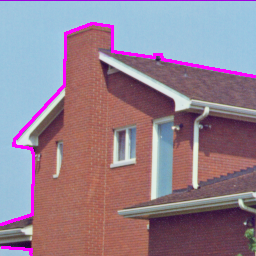
\includegraphics[width=\textwidth]{imgs/granularidade_1}
  \end{subfigure}%
  ~
  \begin{subfigure}[b]{0.3\textwidth}
    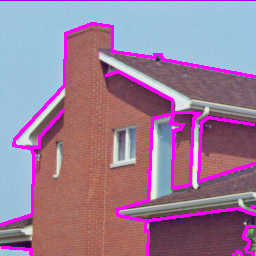
\includegraphics[width=\textwidth]{imgs/granularidade_2}
  \end{subfigure}%
  ~
  \begin{subfigure}[b]{0.3\textwidth}
    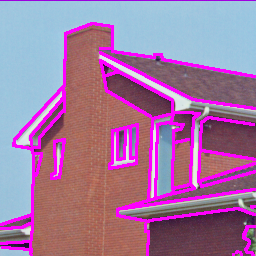
\includegraphics[width=\textwidth]{imgs/granularidade_3}
  \end{subfigure}%
  \caption{Exemplos de uma mesma imagem segmentada de forma consistente, mas com diferentes granularidades de segmentação}
  \label{fig:granularidade}
\end{figure}

Quando a diferença entre duas segmentações advém de uma diferença de percepção da cena, é esperado que o erro seja elevado e que as segmentações sejam consideradas inconsistentes. Quando a diferença é de granularidade, uma segmentação pode ser considerada apenas um refinamento da outra, portanto, o erro deve ser baixo ou até zero \cite{martin:2001}.

Segmentação de imagens é simplesmente a divisão de pixels de uma imagem em conjuntos (segmentos). Uma possível medida de erro tem como entrada duas segmentações, $S_1$ e $S_2$, e tem como saída um valor real no intervalo $[0...1]$, onde $0$ significa ausência de erros de segmentação.

Ainda de acordo com o trabalho de \citeonline{martin:2001}, é necessário utilizar medidas que sejam lenientes com o refinamento de granularidade entre duas segmentações de uma mesma imagem. Entende-se que se os pixels de um segmento podem ser considerados um subconjunto adequado de um outro segmento, trata-se de um refinamento e o erro deve ser zero. Se não existe relação de subconjunto entre os segmentos, as regiões devem ser consideradas inconsistentes e o erro deve ser significativo.

Se $R(S,p_i)$ é o conjunto de pixels correspondentes a uma região na segmentação $S$ que contém o pixel $p_i$, onde $\setminus$ denota o conjunto complementar, o erro de refinamento local é definido por:

\begin{equation}
	\displaystyle E(S_1,S_2,p_i) = \frac{|R(S_1,p_i) \setminus R(S_2,p_i)|}{|R(S_1,p_i)|}
\end{equation}


A partir desta relação, \citeonline{martin:2001} definem duas métricas de erro de segmentação: Erro de Consistência Global (Global Consistency Error, ou GCE) e Erro de Consistência Local (Local Consistency Error, ou LCE):

\begin{equation}
	\displaystyle GCE(S_1,S_2) = \frac{1}{n} min \biggl\{ \sum_{i} E(S_1,S_2,p_i), \sum_{i} E(S_2,S_1,p_i) \biggr\}
\end{equation}

\begin{equation}
	\displaystyle LCE(S_1,S_2) = \frac{1}{n} \sum_{i} min \biggl\{ E(S_1,S_2,p_i), E(S_2,S_1,p_i) \biggr\}
\end{equation}

Uma vez que $LCE \leq GCE$ entre segmentações de uma mesma imagem, é correto afirmar que $GCE$ é uma medida mais rígida que $LCE$. Além dos casos em que uma segmentação é um refinamento de outra, há ainda dois casos em que o erro de segmentação pode ser zero: quando os segmentos são compostos por apenas um pixel cada ou quando toda a imagem é composta de apenas um segmento.

\section{Aprendizagem de máquina e reconhecimento de padrões}

Conforme \citeonline{alpaydin:2010}, aprendizagem de máquina é uma área da inteligência artificial que estuda métodos computacionais, a fim de obter um determinado conhecimento específico através de experiências. A aplicação prática de aprendizado de máquina inclui o processamento de linguagem natural, diagnósticos médicos, detecção de intrusos, entre outros. Um sistema de aprendizado tem a função de analisar informações e generalizá-las, para a extração de novos conhecimentos.

Segundo \citeonline{russell:2010}, os tipos de aprendizagem podem ser classificados de acordo com o tipo de \textit{feedback} que recebem do ambiente:

\begin{itemize}
    \item Aprendizagem não-supervisionada: o agente aprende padrões na entrada, embora não seja fornecido nenhum \textit{feedback} explícito. A tarefa mais comum de aprendizagem não-supervisionada é o agrupamento, ou seja, a detecção de grupos de exemplos de entrada potencialmente úteis.
    \item Aprendizagem por reforço: também conhecida como aprendizagem semi-supervisionada. O agente aprende a partir de uma série de reforços - recompensas ou punições.
    \item Aprendizagem supervisionada: o agente observa alguns exemplos de pares de entrada e saída, e aprende uma função que faz o mapeamento da entrada para a saída.
\end{itemize}

Os problemas de aprendizagem podem ainda ser divididos de acordo com o tipo de saída que demandam:

\begin{itemize}
	\item Problemas de classificação: quando a saída esperada para o problema é uma classe ou categoria, ou seja, um valor discreto;
	\item Problemas de regressão: quando a saída esperada para o problema é um valor numérico, normalmente contínuo.
\end{itemize}

Um problema de classificação consiste na determinação de regras e posterior classificação desses exemplos. Este conjunto de regras é criado por um classificador, que recebe como entrada um vetor de características e oferece como saída uma classe resultante para a instância que as características descrevem, conforme pode ser visto na figura \ref{fig:classificador}.

\begin{figure}[h!]
  \centering
  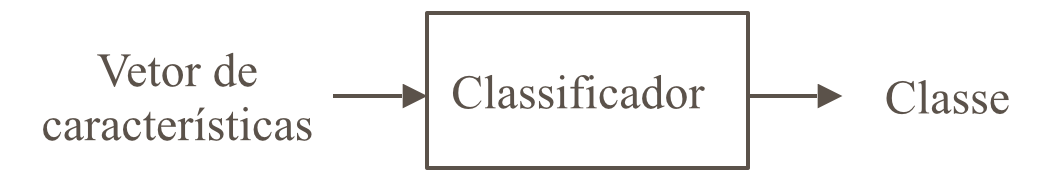
\includegraphics[width=0.7\textwidth]{imgs/classificador}
  \caption{Representação de classificador como uma função de bloco}
  \label{fig:classificador}
\end{figure}

Os tipos de classificadores utilizados neste trabalho serão discutidos com mais detalhes na seção \ref{sec:classificacao}.

Para a composição do modelo de aprendizagem, uma base de dados de treinamento é utilizada. Esta base deve possuir uma quantidade significativa e com boa representatividade das classes envolvidas no problema. Normalmente se usa uma parte da base de dados de treinamento para validação do modelo de aprendizado (validação cruzada) ou mesmo uma base de dados diferente (base de testes ou validação), para que indicadores de qualidade do modelo possam ser avaliados. A seção \ref{sec:avaliacao} discorre sobre os métodos de avaliação utilizados neste trabalho.

Técnicas de aprendizagem de máquina podem ser utilizadas para encontrar padrões em diversos domínios, inclusive em imagens. É neste ponto que a linha de pesquisa de aprendizagem de máquina, advinda da área de inteligência artificial, se encontra com a linha de pesquisa de reconhecimento de padrões, advinda da área de processamento de sinais. Segundo \citeonline{jain:1989}, o fluxo padrão para soluções de reconhecimento de padrões consiste em três etapas:

\begin{enumerate}
    \item Filtragem e pré-processamento da entrada;
    \item Extração e seleção de características;
    \item Classificação.
\end{enumerate}


\subsection{Filtragem e Pré-processamento}

A etapa de filtragem e pré-processamento é responsável pela escolha e montagem da base de dados que será usada no processo de aprendizagem. A base deve conter uma quantidade significativa de exemplos de todas as classes envolvidas no problema.

Em aprendizado relacionado a imagens, essa etapa é comumente a responsável por normalizar e salientar as características desejadas nas amostras (realce de imagens, filtragem, etc). Exemplos irrelevantes, distorcidos ou repetidos também são eliminados durante a filtragem. O objetivo principal desta etapa é preparar a base de dados para as etapas seguintes.


\subsection{Extração e Seleção de Características}

A extração de características é feita selecionando os atributos oriundos dos dados (imagens, no trabalho em questão), a fim de encontrar as características úteis para o processo de reconhecimento. Essa etapa é crítica ao sucesso do aprendizado, uma vez que bons algoritmos de aprendizado só obtêm êxito com um bom conjunto de características relevantes ao problema.

Em projetos que envolvem classificação de imagens, uma gama de atributos pode ser extraída, e podem ser descritos pelo nível da informação que representam. Nesta etapa há uma forte contribuição da linha de pesquisa de processamento digital de imagens \cite{gonzalez:2002}, que descreve filtragens, transformações e outras técnicas capazes de extrair informações sobre uma imagem ou pedaços dela.

Segundo \citeonline{nixon:2008}, características de baixo nível como bordas, histogramas de intensidade e coloração, são úteis para o reconhecimento de padrões em imagens, assim como características de níveis mais altos, como texturas, transformadas de Hough e extração de regiões conectadas.

Em um estágio inicial de uma solução de aprendizagem de máquina, é natural que sejam utilizadas grandes quantidades de características para descrever as amostras. Com o avanço da pesquisa e análise de resultados parciais, é esperado que a dimensionalidade deste vetor diminua. Isto é desejado por dois motivos: a alta dimensionalidade do vetor de características tem impacto significativo no desempenho computacional de vários algoritmos de aprendizagem de máquina e a presença de atributos que possuam pequena contribuição para a classificação podem causar ruído no aprendizado, dificultando sua generalização. Estes dois problemas serão abordados com mais detalhes nas seções \ref{sec:classificacao} e \ref{sec:avaliacao}.

Uma técnica bastante difundida para a seleção de características em problemas de aprendizagem de máquina supervisionada é a \textit{Correlation-based Feature Selection} (CFS), introduzida por \citeonline{hall:1998}. A idéia geral desta técnica é a avaliação de quais atributos são bons ou ruins para um determinado conjunto de dados supervisionados. Bons atributos possuem alta correlação com a classe da amostra, e ao mesmo tempo, baixa correlação com os demais atributos da mesma amostra. Formalmente, um atributo $V_i$ é considerado relevante se, e somente se, existe um $v_i$ e $c$ para os quais $p(V_i = v_i) > 0$ de tal maneira que:

\begin{equation}
	\displaystyle p(C=c|V_i=v_i) \neq p(C=c)
\end{equation}

onde $p(C=c|V_i=v_i)$ é a probabilidade condicional de que a classe $C$ de uma amostra é $c$ dado que o valor do atributo $V_i$ é $v_i$.

O produto desta etapa é a representação de cada exemplo da base de dados em um vetor de características, de forma que possa ser usado por um ou mais classificadores em uma etapa posterior.


\subsection{Classificação}\label{sec:classificacao}

Nesta etapa, um modelo de aprendizado é gerado. Pode-se também usar múltiplos classificadores, ao invés de apenas um. Esta abordagem é chamada de sistemas com múltiplos classificadores (do inglês \textit{multiple classifier systems}), também chamados de \textit{ensemble} de classificadores, os quais podem ser compostos por classificadores do mesmo tipo ou de diferentes algoritmos de classificação.

Existe uma grande variedade de algoritmos de aprendizagem de máquina propostos na literatura. Alguns dos mais utilizados são: classificadores estatísticos, redes neurais artificiais, árvores de decisão, máquinas de vetores de suporte (SVM), k vizinhos mais próximos (KNN), etc. A seguir, descrevemos sucintamente os algoritmos de aprendizagem de máquina utilizados neste trabalho.

\subsubsection*{Árvores de decisão}

Amplamente utilizadas em algoritmos de classificação, as árvores de decisão são representações simples do conhecimento e um meio eficiente de construir classificadores que predizem classes baseadas nos valores de atributos de um conjunto de dados. As árvores de decisão consistem de nodos que representam os atributos; de arcos, provenientes destes nodos e que recebem os valores possíveis para estes atributos; e de nodos folha, que representam as diferentes classes de um conjunto de treinamento. Classificação, neste caso, é a construção de uma estrutura de árvore, que pode ser usada para classificar corretamente todos os objetos do conjunto de dados da entrada.

A partir de uma árvore de decisão é possível derivar regras. As regras são escritas considerando o trajeto do nodo raiz até uma folha da árvore. Estes dois métodos são geralmente utilizados em conjunto. Devido ao fato das árvores de decisão tenderem a crescer muito, de acordo com algumas aplicações, elas são muitas vezes substituídas pelas regras. Isto acontece em virtude das regras poderem ser facilmente modularizadas. Uma regra pode ser compreendida sem que haja a necessidade de se referenciar outras regras.

Uma árvore de decisão tem a função de particionar recursivamente um conjunto de treinamento, até que cada subconjunto obtido deste particionamento contenha casos de uma única classe. Para atingir esta meta, a técnica de árvores de decisão examina e compara a distribuição de classes durante a construção da árvore. O resultado obtido, após a construção de uma árvore de decisão, são dados organizados de maneira compacta, que são utilizados para classificar novos casos. A árvore de decisão não presume nenhum modelo estatístico a priori, sendo a divisão do espaço de atributos feita de acordo com as amostras provenientes do treinamento.

\subsubsection*{KNN}

O algoritmo KNN (K-Nearest Neighbours, ou K vizinhos mais próximos) \cite{cover:1967} é um método de classificação baseado na proximidade de amostras de treino no espaço de características. É considerado um dos mais simples algoritmos de aprendizagem de máquina.

O processo de treinamento para esse algoritmo consiste em armazenar o vetor de característica e rótulos (classes) de cada amostra de treinamento em um espaço n-dimensional, onde n é o número de características de cada amostra. No processo de classificação de amostras não-rotuladas, a amostra é simplesmente projetada no espaço e é classificada de acordo com as k amostras mais próximas.

Quando k = 1, a amostra é simplesmente classificada de acordo com o rótulo de seu vizinho mais próximo no espaço de características. Quando k é maior que 1, a classificação se dá por um esquema de votação, onde a classe com as amostras vizinhas mais numerosas é considerada como a classe da amostra. Por essa razão, em problemas bi-classe como o apresentado nesta dissertação, deve ser utilizado um valor ímpar para $k$, com a finalidade de evitar empates. Em problemas multi-classe, ou seja, com mais de duas classes possíveis, empates podem acontecer mesmo considerando um número ímpar de vizinhos, de maneira que uma forma de desempate deve ser definida na implementação do algoritmo.

Diversas formas de calcular a distância entre duas amostras $a$ e $b$ em um espaço n-dimensional podem ser utilizadas no kNN, dentre elas a distância Euclidiana, representada pela fórmula \ref{eq:euclides}, onde $n$ é o número de dimensões.

\begin{equation}
	\displaystyle d(a,b) = ||a - b|| = \sqrt{(a - b)*(a -b)} =
	\displaystyle \sqrt{\sum_{i=1}^{n}(a_i - b_i)^2}
\label{eq:euclides}
\end{equation}

\subsubsection*{Support Vector Machines}

As máquinas de vetores de suporte, ou SVM (\textit{Support Vector Machines}) são classificadores baseados na teoria de aprendizagem estatística proposta por \cite{vapnik:1995}. A teoria é baseada em uma forte fundamentação matemática para estimação de dependências e previsão do aprendizado a partir de conjuntos de dados finitos. 

Um modelo SVM é a representação das amostras como pontos em um espaço n-dimensional (onde n é o tamanho do vetor de características) de tal forma que as amostras de diferentes classes sejam divididas por um hiperplano de separação que maximiza a distância entre essas classes. Isso se deve ao fato de que o hiperplano de separação possui a maior distância possível às amostras mais próximas entre as classes, o que ajuda a diminuir o erro de generalização do classificador.

A principal vantagem do classificador SVM é seu bom desempenho em conjuntos de dados que possuem muitos atributos, mesmo quando há poucas amostras de treino. No entanto, suas desvantagens são a baixa velocidade e alto consumo de recursos durante as fases de treinamento, assim como a complexidade de parametrização de suas funções \textit{kernel}. As amostras desconhecidas são classificadas ao serem posicionadas no espaço de características e avaliadas em que lado da superfície de separação elas se encontram, como mostrado na figura \ref{fig:svm}.

\begin{figure}[h!]
  \centering
  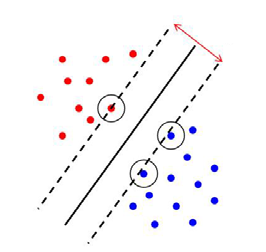
\includegraphics[scale=0.5]{imgs/svm}
  \caption[Máquina de vetores de suporte]{Amostras em um espaço bidimensional (pontos coloridos) separadas por um hiperplano apoiado por vetores de suporte (pontos circulados), maximizando a distância entre as amostras mais próximas do limiar das classes.}
  \label{fig:svm}
\end{figure}

\subsubsection*{Naive Bayes}

Há um grupo de algoritmos de aprendizado de máquina que se baseiam em raciocínio probabilístico, especialmente sob o viés bayseano. De acordo com \citeonline{mitchell:1997}, o raciocínio bayesiano é baseado no pressuposto de que as quantidades de interesse são governadas pela distribuição das probabilidade e que decisões ótimas podem ser tomadas a partir da análise destas probabilidades em conjunto com os dados observados.

O teorema de Bayes estabelece a relação entre uma probabilidade condicional e sua probabilidade inversa. A equação \ref{eq:teoremaDeBayes}, conhecida como regra de Bayes, permite calcular a probabilidade de um evento (A) dado que outro evento aconteceu (B).

\begin{equation}
	\displaystyle P(A|B) = \frac{P(B|A) P(A)}{P(B)}
\label{eq:teoremaDeBayes}
\end{equation}

A probabilidade \textit{a priori}, ou seja, a probabilidade isolada de que um evento $A$ aconteça é expressa por $P(A)$. A probabilidade \textit{a posteriori} de um evento $A$ dado que ocorreu também um evento $B$ é expressa por $P(A|B)$.

Dentre as técnicas de inspiração probabilística, \textit{Naive Bayes} se destaca por sua simplicidade. Apresentada por \citeonline{john:1995}, esta família de algoritmos presume uma forte independência entre as variáveis do vetor de características, por isso é chamado de Bayes Ingênuo (do inglês \textit{Naive Bayes}).

Segundo \citeonline{russell:2010}, os valores de máxima probabilidade de cada classe de acordo com as variáveis do vetor de características são encontrados. Uma vez que um modelo é gerado desta maneira, as futuras amostras podem ser classificadas de acordo com as mesmas probabilidades. Dado que o vetor de características das amostras é denotado por $x_1, x_2,...,x_n$, a probabilidade de cada classe C é expressa pela equação \ref{eq:probabilidadeNaiveBayes}. A família de algoritmos \textit{Naive Bayes} tende a ser bastante robusta em face a dados ruidosos ou ausentes.

\begin{equation}
	\displaystyle P(C|x_1,x_2,...,x_n) = P(C) \prod_{i}{P(x_i|C)}
\label{eq:probabilidadeNaiveBayes}
\end{equation}

\subsubsection*{Random Forest}

O algoritmo \textit{Random Forest}, introduzido por \citeonline{breiman:2001} , é um \textit{ensemble} de classificadores de árvore de decisão. Na fase de treinamento, um número determinado de árvores é gerado utilizando um subconjunto pseudo-aleatório do vetor de características completo utilizado no problema. Tanto o número de árvores quanto a quantidade de atributos utilizados por cada árvore pode ser determinado pelo usuário do algoritmo.

Uma vez que a base de treinamento foi utilizada para gerar os modelos das árvores de decisão, estes modelos podem ser utilizados para classificar novas amostras do problema. Preferencialmente, todas as árvores geradas são envolvidas na classificação, cada uma chegando à sua própria conclusão sobre a classe da amostra apresentada. Cada árvore tem um ``voto'', que é contabilizado para a definição da classe mais votada, que é então escolhida como a classe da amostra. Esta técnica de soma de votos é conhecida como \textit{polling}.

A principal vantagem deste algoritmo é a eliminação de \textit{overfitting}, problema bastante comum quando se utiliza árvores de decisão de forma tradicional. Uma exposição mais detalhada acerca de \textit{overfitting} é feita na seção \ref{sec:avaliacao}. O trabalho de \citeonline{breiman:2001} ainda afirma que a taxa de erro de um modelo de aprendizado criado com \textit{Random Forest} está relacionada a dois fatores: a correlação entre quaisquer duas árvores geradas no modelo e a ``força'' de cada árvore gerada, ou seja, o quão precisa cada árvore é em relação ao modelo geral. À medida que a correlação entre árvores cresce, também cresce a taxa de erro do modelo final. Quanto menor for a taxa de erro de uma árvore individual, mais ``forte'' é considerado o classificador, e por consequência, menor é a taxa de erro do modelo.

Reduzir o número de variáveis do vetor de características a ser utilizado em cada árvore reduz a correlação entre árvores e também reduz a ``força'' da árvore. Incrementar este número de variáveis incrementa a correlação e a ``força'' da árvore. A parametrização do algoritmo deve se preocupar em encontrar o número de variáveis do vetor de características que melhor minimize a correlação e maximize a ``força'' das árvores do modelo.

Os algoritmos descritos até então podem ser utilizados em qualquer problema de classificação binária ou multi-classe. Entretanto, há um grupo de algoritmos em aprendizagem de máquina que tem como objetivo a detecção de anomalias a partir de um modelo formado por apenas uma classe. A próxima seção trata desta classe de algoritmos.

\subsubsection*{Classificadores unários}

Algoritmos conhecidos como classificadores unários são utilizados, normalmente, em problemas onde há apenas uma classe conhecida, e há interesse em se encontrar anomalias ou novidades, ou seja, amostras que não pertencem à classe conhecida.

 Neste tipo de problema, a base é normalmente composta por uma única classe (conhecida como classe alvo, ou \textit{target}) e o modelo gerado é supostamente capaz de determinar se novas amostras do problema pertencem à classe alvo ou se são anomalias ou novidades (\textit{outliers}). Estes algoritmos também são chamados de detectores de novidades (\textit{novelty detection}) ou detectores de anomalias (\textit{outlier detection}).

Apesar de serem concebidos para problemas de classificação de apenas uma classe, algoritmos de detecção de anomalias podem ser utilizados para resolução de problemas com múltiplas classes. A estratégia consiste em treinar um classificador deste tipo para cada classe do problema. Diversas técnicas para apuração dos resultados podem ser utilizadas, tais como votação (\textit{voting} ou \textit{polling}), onde cada classificador tem um voto que é computado com um peso e levado em consideração na classificação final; ou bagging (abreviação do termo inglês \textit{Bootstrap aggregating}), que se utiliza da combinação do resultado de classificação de conjuntos de dados de treinamento selecionados aleatoriamente, com o objetivo de reduzir a variância e o \textit{overfitting}, discutidos com mais detalhes na seção \ref{sec:avaliacao}.

Uma variante do SVM denominada OC-SVM (acrônimo em inglês para \textit{One Class Support Vector Machines}) foi introduzida por \citeonline{scholkopf:1999} com a finalidade de adaptar o robusto algoritmo de \citeonline{vapnik:1995} para problemas de detecção de anomalias. Este é, na verdade, uma expansão da aplicação da técnica de SVM para dados não-rotulados.

A ideia central é que uma função \textit{kernel} de base radial é utilizada para comportar as amostras da classe alvo, de forma a medir a possibilidade de anomalias futuras de acordo com a distância destas mesmas amostras em relação à hiperesfera de separação descrita pela função \textit{kernel}. Em uma problema com múltiplas classes e classificadores OC-SVM, costuma-se usar uma estratégia de votação com pesos para determinação da classe da amostra.

Outros métodos tradicionais em problemas multi-classe também podem ser usados como classificadores para detecção de anomalias. Variações de KNN como o OCNN (\textit{One-Class Nearest Neighbour}) ou de árvores de decisão como o REPTree são comumente utilizados nesta abordagem, utilizando diversas estratégias para determinação final das classes das novas amostras.

Há ainda na literatura trabalhos que descrevem modelos para utilização de diversos algoritmos unários diferentes em um mesmo problema, definindo também estratégias para a determinação da classificação resultante da miríade de classificadores. Isto possibilita um grau de liberdade elevado na escolha desses algoritmos e estratégias para problemas multi-classe.

Tanto durante o desenvolvimento de uma solução, quanto após sua execução em ambiente de produção, é preciso aferir e quantificar o desempenho da técnica desenvolvida ou utilizada, conforme discutido na próxima seção.

\subsection{Avaliação de aprendizagem}\label{sec:avaliacao}

Avaliar o desempenho de uma técnica de aprendizagem de máquina é útil para determinar a qualidade do modelo criado, aferir se o modelo continua adequado e inspecionar se os atributos escolhidos são relevantes para a classificação das amostras.

Comumente, o percentual de acerto obtido na classificação das amostras é um importante parâmetro para medir o desempenho do modelo. Este parâmetro é conhecido como acurácia ou taxa de reconhecimento. O oposto da acurácia é conhecido como taxa de erro.

De grande importância também é a composição da matriz de confusão (tabela \ref{tab:matrixConfusao}). Nela pode-se avaliar como um modelo está se comportando em termos de falsos positivos (um exemplo é classificado como pertencente à classe C, mas não é) e falsos negativos (um exemplo é atribuído a outra classe, mas deveria ser da classe C). A principal função desta matriz é dar possibilidade de pensar sobre o custo dos erros, ou seja, mesmo que a taxa de acerto para o problema seja alta, uma ou mais classes do problema pode ter uma taxa de acerto bem abaixo do esperado.

\begin{table}[h]
  \centering
  \begin{tabular}{cccc}
  \multicolumn{2}{c}{\textbf{Resultado obtido}}                  &                               &                                              \\ \cline{1-2}
  \multicolumn{1}{|c|}{Classe A} & \multicolumn{1}{c|}{Classe B} &                               &                                              \\ \cline{1-3}
  \multicolumn{1}{|c|}{Verdadeiro positivo}       & \multicolumn{1}{c|}{Falso negativo}       & \multicolumn{1}{c|}{Classe A} & \multirow{2}{*}{\textbf{Resultado esperado}} \\ \cline{1-3}
  \multicolumn{1}{|c|}{Falso positivo}       & \multicolumn{1}{c|}{Verdadeiro negativo}       & \multicolumn{1}{c|}{Classe B} &                                              \\ \cline{1-3}
  \end{tabular}
  \caption{Modelo de matriz de confusão.}
  \label{tab:matrixConfusao}
\end{table}

Alguns valores podem ser obtidos através desta matriz. A própria acurácia do modelo pode ser obtida com a equação \ref{eq:acuracia}, onde TP representa o número de verdadeiros positivos, FP representa os falsos positivos, FN representa os falsos negativos e TN representa os verdadeiros negativos.

\begin{equation}
  \displaystyle Acurácia = \frac{TP+TN}{TP+FP+TN+FN}
\label{eq:acuracia}
\end{equation}

Ainda é possível obter a precisão e a revocação. A precisão é o número de elementos relevantes recuperados dividido pelo número total de elementos recuperados (equação \ref{eq:precisao}) enquanto a revocação é definida como o número de elementos relevantes recuperados dividido pelo número total de elementos relevantes existentes, que deveriam ter sido recuperados (equação \ref{eq:revocacao}).

\begin{equation}
  \displaystyle Precisão = \frac{TP}{TP+FP}
\label{eq:precisao}
\end{equation}

\begin{equation}
  \displaystyle Revocação = \frac{TP}{TP+FN}
\label{eq:revocacao}
\end{equation}

Como forma de medir o equilíbrio entre precisão e revocação, a média harmônica entre estas duas medidas é calculada. Esta medida é chamada de $F_1$ ($F_1$ \textit{score}, em inglês), e é obtida a partir da equação \ref{eq:f1}.

\begin{equation}
  \displaystyle F_1 = 2 \cdot \frac{precisão \cdot revocação}{precisão + revocação}
\label{eq:f1}
\end{equation}

Embora a maximização das métricas apresentadas seja desejável para o ajuste de um algoritmo de aprendizado, é necessário evitar o sobreajuste (\textit{overfitting}) que pode ser gerado a partir disto. O \textit{overfitting} é o termo utilizado quando o modelo criado se ajusta em excesso às amostras de treinamento, tendo altas taxas de acurácia para esta base, mas falhando em classificar com boa taxa de acurácia as demais amostras de teste ou amostras reais. Em resumo, o problema é ter um modelo que possui bom desempenho na etapa de treinamento mas não é uma boa representação das amostras reais.

%A figura \ref{fig:overfitting} exemplifica um modelo de classificação generalista (linha preta) e um modelo que provavelmente sofre de \textit{overfitting} (linha verde).
%
%\begin{figure}[h!]
%  \centering
%  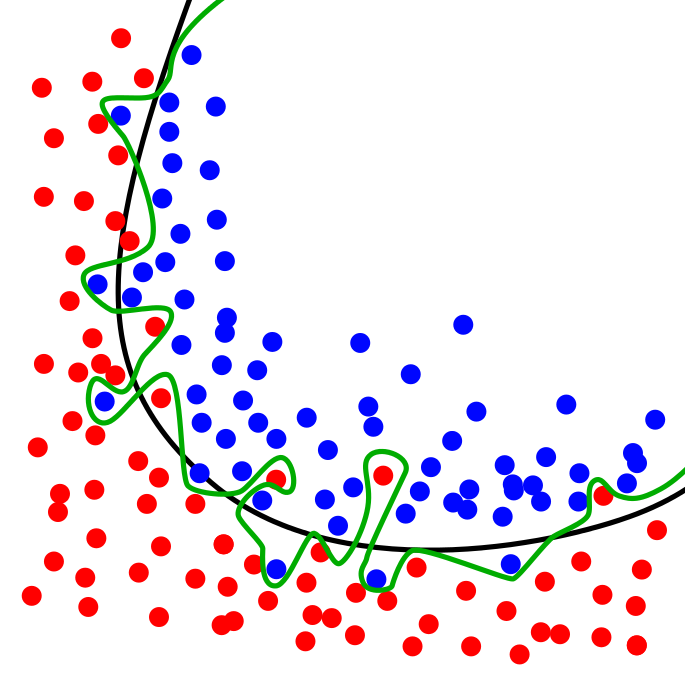
\includegraphics[scale=0.4]{imgs/overfitting}
%  \caption[Modelo de aprendizado generalista]{Modelo de aprendizado em um problema de duas classes, a linha preta indica uma função mais generalista, enquanto a linha verde representa uma função com acurácia maior em relação às amostras de treinamento, mas que provavelmente sofre de \textit{overfitting.}}
%  \label{fig:overfitting}
%\end{figure}
%
%Para detectar problemas de \textit{overfitting}, pode-se testar o modelo em diversas outras bases de amostras, medindo a variância da acurácia entre estas bases. Uma alta variância indica que o modelo não é genérico o suficiente, apontando para um provável caso de \textit{overfitting}.

Um método bastante utilizado para medir a generalização de um modelo de aprendizado é a validação cruzada. O conceito principal deste método é o particionamento do conjunto de amostras em um número de subconjuntos mutuamente exclusivos, divindindo estes subconjuntos entre base de treinamento e teste.

A técnica de validação cruzada conhecida como \textit{k-fold} divide a base em $k$ subconjuntos de mesmo tamanho, escolhe um dos subconjuntos como base de testes e utiliza os demais subconjuntos como bases de treinamento do modelo. A razão para estar distribuição é a premissa de que é preciso de mais amostras para treinamento que para testes, a fim de criar um modelo robusto. O procedimento é repetido $k$ vezes, de forma que todos os subconjuntos possam ser utilizados para construir uma versão de modelo de aprendizado e ser validado pelos demais subconjuntos.

%A precisão do modelo é obtida através de uma média aritmética simples das $k$ execuções da validação cruzada. Em problemas de regressão, a precisão do modelo é obtida pela equação \ref{eq:kfold}, onde $k$ é o número de subconjuntos e $y_i - y'_i$ é a diferença entre o valor esperado e o valor predito pelo modelo.
%
%\begin{equation}
%  \displaystyle Ac_f = \frac{1}{k} \sum_{i=1}^k{(y_i - y'_i)}
%\label{eq:kfold}
%\end{equation}
%
%Segundo \citeonline{witten:2011}, é prática comum repetir a execução da validação \textit{k-fold}, por $k$ vezes. A razão disto é o efeito provocado pela variação na escolha dos subconjuntos de treinamento e teste, que ocasiona pequenas variações nas taxas de erro e precisão entre diferentes execuções de um mesmo modelo no mesmo conjunto geral de dados. A execução de $k^2$ validações tende a diminuir esta variação, ao custo de um esforço computacional mais intenso.

Uma outra avaliação importante a ser feita é a da relação entre a taxa de acerto (verdadeiros positivos) e  a taxa de falsos positivos. Para tal análise, pode ser feito o estudo da curva ROC (do inglês \textit{Receiver Operating Characteristic}), um gráfico bidimensional que exibe no eixo y o percentual de verdadeiros positivos na amostra e, no eixo x, o percentual de falsos positivos da mesma amostra (figura \ref{fig:roc}).

\begin{figure}[h]
  \centering
  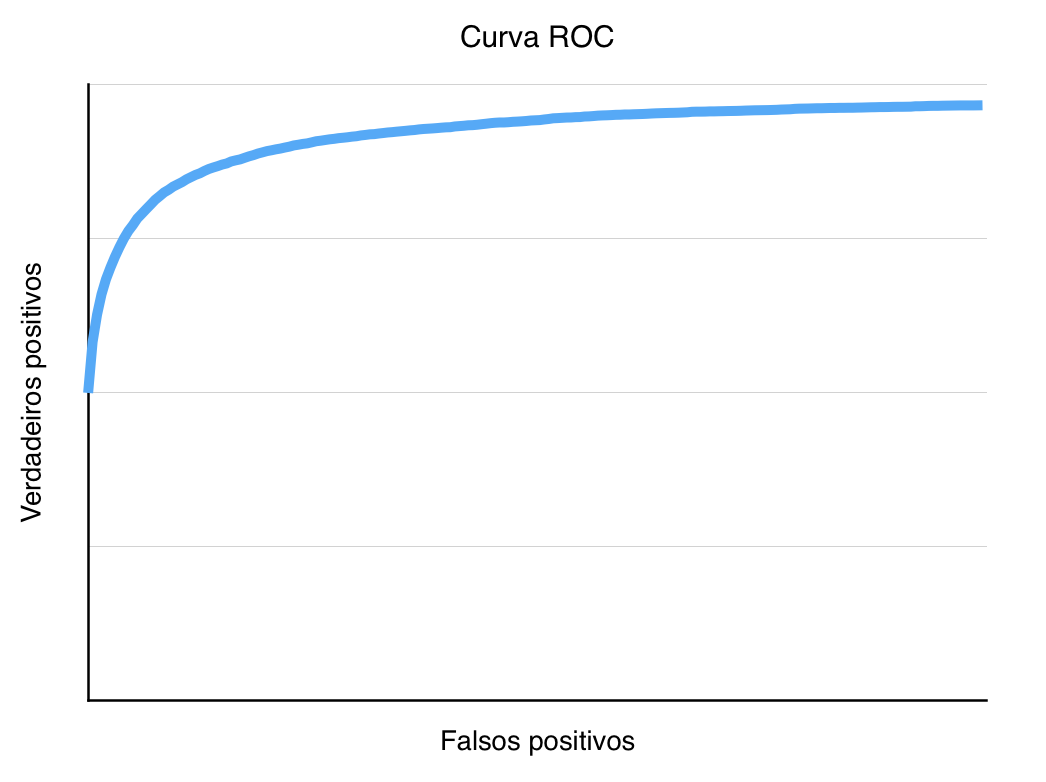
\includegraphics[scale=0.6]{imgs/roc}
  \caption{Exemplo de gráfico para análise de curva ROC.}
  \label{fig:roc}
\end{figure}

Originalmente utilizada em detecção de sinais para mostrar a relação entre sensibilidade (taxa de acerto) e o inverso da especificidade (alarme falso) em canais com ruído, pode-se utilizar este gráfico na avaliação de modelos de aprendizagem de máquina. Em geral, o cálculo da área abaixo da linha do gráfico é realizado para determinar a relação entre verdadeiros positivos e falsos negativos para um conjunto de amostras. Quanto maior a área abaixo da curva, melhor é considerado o aprendizado sob esta avaliação.

Uma vez que a fundamentação teórica necessária foi coberta, é necessário fazer um levantamento na literatura pelos trabalhos considerados estado da arte em suas respectivas áreas. O capítulo a seguir trata deste levantamento.